\documentclass[11pt]{article}

\usepackage[margin=0.82in]{geometry}
\usepackage{graphicx}
\usepackage{booktabs}
\usepackage{array}
\usepackage{xcolor}
\usepackage{amsmath}
\usepackage{caption}
\usepackage[hidelinks]{hyperref}

\definecolor{accent}{HTML}{2A9D8F}
\definecolor{warn}{HTML}{E76F51}
\definecolor{muted}{HTML}{4C556A}

\title{\vspace{-1.0cm}\textbf{TinyGRPO-Math: Rule-Based GRPO Post-Training on GSM8K}}
\author{Yashas Kotre}
\date{\today}

\begin{document}
\maketitle
\vspace{-0.5cm}

\begin{abstract}
This report evaluates a compact GRPO post-training experiment for mathematical reasoning on GSM8K. A non-math-specialized base model, \texttt{Qwen/Qwen2.5-1.5B-Instruct}, was trained with deterministic rule-based rewards instead of a learned reward model. The reward combines exact final-answer correctness, final-line answer formatting, parseability, and penalties for invalid or overlong outputs. On 200 held-out GSM8K test examples, the 1000-update continuation model improved accuracy from \textbf{66.5\%} to \textbf{71.0\%} and final-answer format compliance from \textbf{77.5\%} to \textbf{97.5\%}, while preserving 100\% parseability and zero truncation.
\end{abstract}

\section{Experiment Summary}

\textbf{Goal.} Adapt a from-scratch GRPO training loop from preference-style chatbot alignment to verifiable math reasoning. GSM8K is a good fit because final answers are objective and can be scored without training a reward model.

\textbf{Model.} The policy and KL reference use \texttt{Qwen/Qwen2.5-1.5B-Instruct}. I intentionally did not use a math-specialized checkpoint as the training target, since an already math-post-trained model would leave less room for visible improvement.

\textbf{Data.} Training used GSM8K train rows 0--999 in two stages. Evaluation used GSM8K test rows 0--199. An exact question-text overlap check between these 1000 train questions and 200 test questions found 0 overlaps.

\textbf{Training.} Each GRPO update sampled \(G=4\) completions for one prompt. The first stage trained on rows 0--499 for 500 updates. The continuation stage initialized the policy from the first stage checkpoint, kept the KL reference anchored to the original base model, and trained on rows 500--999 for another 500 updates. The continuation stage used a lower learning rate to reduce destructive drift.

\begin{table}[h]
\centering
\caption{Training configuration.}
\begin{tabular}{lll}
\toprule
Setting & Stage 1 & Stage 2 continuation \\
\midrule
Policy initialization & Base model & Stage 1 checkpoint \\
KL reference & Base model & Base model \\
Train rows & 0--499 & 500--999 \\
Updates & 500 & 500 \\
Group size & 4 & 4 \\
Learning rate & \(5\times 10^{-6}\) & \(2\times 10^{-6}\) \\
KL beta & 0.05 & 0.05 \\
Sampling & temperature 0.7, top-p 0.95 & temperature 0.7, top-p 0.95 \\
\bottomrule
\end{tabular}
\end{table}

\section{Reward Design}

The reward is deterministic and rule-based. The dominant signal is final-answer correctness, with smaller shaping terms for parseable and consistently formatted outputs.

\begin{table}[h]
\centering
\caption{Reward components.}
\begin{tabular}{ll}
\toprule
Condition & Reward contribution \\
\midrule
Final answer numerically correct & +1.0 \\
Completion ends with a recognized final answer line & +0.2 \\
Answer is parseable as a number or expression & +0.1 \\
Parseable answer is wrong & -0.4 \\
No parseable answer & -0.5 \\
Completion exceeds character budget & -0.2 \\
Generation reaches max length without EOS & -0.3 \\
\bottomrule
\end{tabular}
\end{table}

The intended format is a final line of the form \texttt{Answer: <number>}. The scorer also accepts common variants such as \texttt{Final Answer: <number>} and boxed LaTeX answers as fallbacks. Numeric equality handles commas, currency symbols, decimal/integer equivalence, fractions, and simple LaTeX fractions. If \texttt{math-verify} is installed, it is used as an additional correctness verifier.

\section{Held-Out Results}

Table~\ref{tab:eval} compares the base model, the 500-update model, and the 1000-update continuation model on the same 200 held-out GSM8K test examples.

\begin{table}[h]
\centering
\caption{Held-out GSM8K test performance on 200 examples.}
\label{tab:eval}
\begin{tabular}{lrrrrr}
\toprule
Model & Correct & Accuracy & Answer format & Parseable & Avg. reward \\
\midrule
Base & 133/200 & 66.5\% & 155/200, 77.5\% & 200/200 & 0.786 \\
GRPO-500 & 140/200 & 70.0\% & 196/200, 98.0\% & 200/200 & 0.876 \\
GRPO-1000 & 142/200 & 71.0\% & 195/200, 97.5\% & 200/200 & 0.889 \\
\bottomrule
\end{tabular}
\end{table}

Relative to the base model, GRPO-1000 improved accuracy by \textbf{+4.5 percentage points} and answer-format compliance by \textbf{+20.0 percentage points}. Truncation remained 0/200 for all runs.

\begin{figure}[h]
\centering
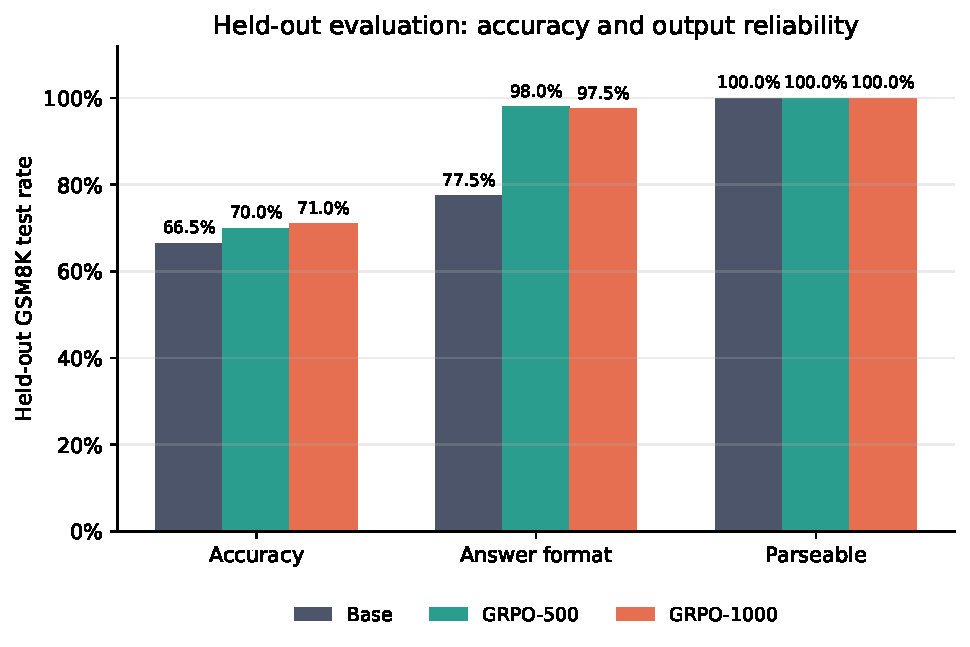
\includegraphics[width=0.92\linewidth]{figures/eval_metrics.pdf}
\caption{Accuracy, final-answer format compliance, and parseability on held-out GSM8K examples.}
\end{figure}

\begin{figure}[h]
\centering
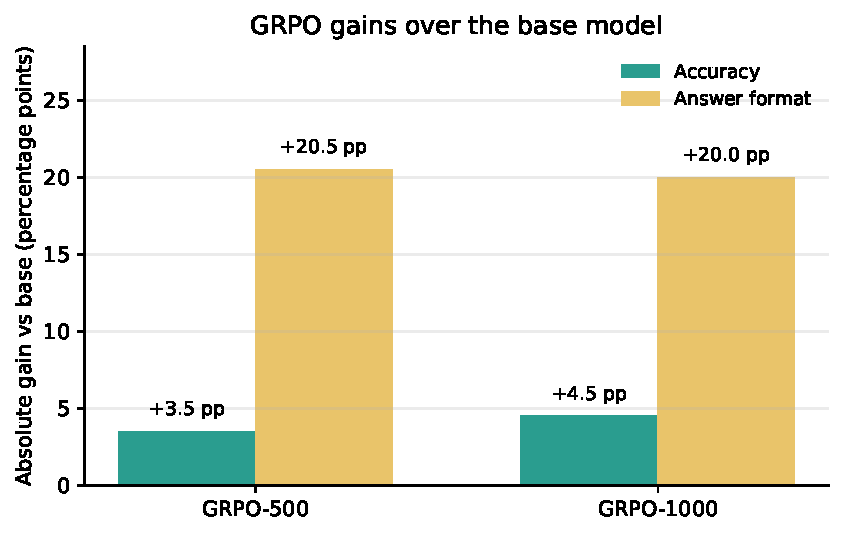
\includegraphics[width=0.82\linewidth]{figures/eval_deltas.pdf}
\caption{Absolute gains over the base model. The largest gain is in final-answer format compliance, but accuracy also improves.}
\end{figure}

\section{Paired Flip Analysis}

Because every model was evaluated on the same 200 test examples, the most useful comparison is paired: which examples changed from wrong to correct, and which regressed?

\begin{table}[h]
\centering
\caption{Paired correctness flips versus the base model.}
\resizebox{\linewidth}{!}{%
\begin{tabular}{lrrrrr}
\toprule
Model & Both correct & Base wrong, trained correct & Base correct, trained wrong & Both wrong & Net gain \\
\midrule
GRPO-500 & 118 & 22 & 15 & 45 & +7 \\
GRPO-1000 & 118 & 24 & 15 & 43 & +9 \\
\bottomrule
\end{tabular}
}
\end{table}

For GRPO-1000, 24 examples improved from wrong to correct, while 15 regressed from correct to wrong, giving a net gain of 9 examples. This matches the aggregate gain from 133/200 to 142/200. A conservative exact paired sign test on the 39 discordant examples gives \(p=0.200\), so this should be presented as a promising pilot result rather than a statistically conclusive benchmark result.

\begin{figure}[h]
\centering
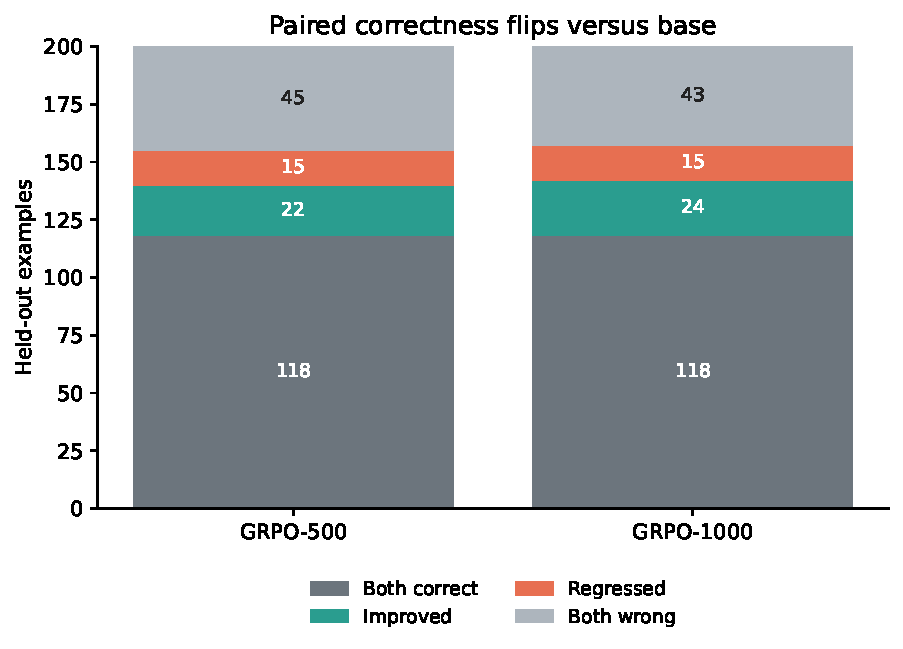
\includegraphics[width=0.82\linewidth]{figures/paired_flips.pdf}
\caption{Paired correctness outcomes versus the base model.}
\end{figure}

\section{Training Dynamics}

The training logs show that the model learned the requested output format quickly and maintained stable GPU behavior. The continuation stage achieved higher train-time completion correctness, but the held-out accuracy gain from Stage 1 to Stage 2 was modest.

\begin{table}[h]
\centering
\caption{Training-time completion statistics.}
\resizebox{\linewidth}{!}{%
\begin{tabular}{lrrrrr}
\toprule
Run & Sampled completions & Correct completions & Format compliance & Avg. step reward & Truncated \\
\midrule
GRPO-500 & 2000 & 1401, 70.1\% & 1753, 87.7\% & 0.856 & 0 \\
Continuation & 2000 & 1547, 77.4\% & 1862, 93.1\% & 0.969 & 0 \\
\bottomrule
\end{tabular}
}
\end{table}

\begin{figure}[h]
\centering
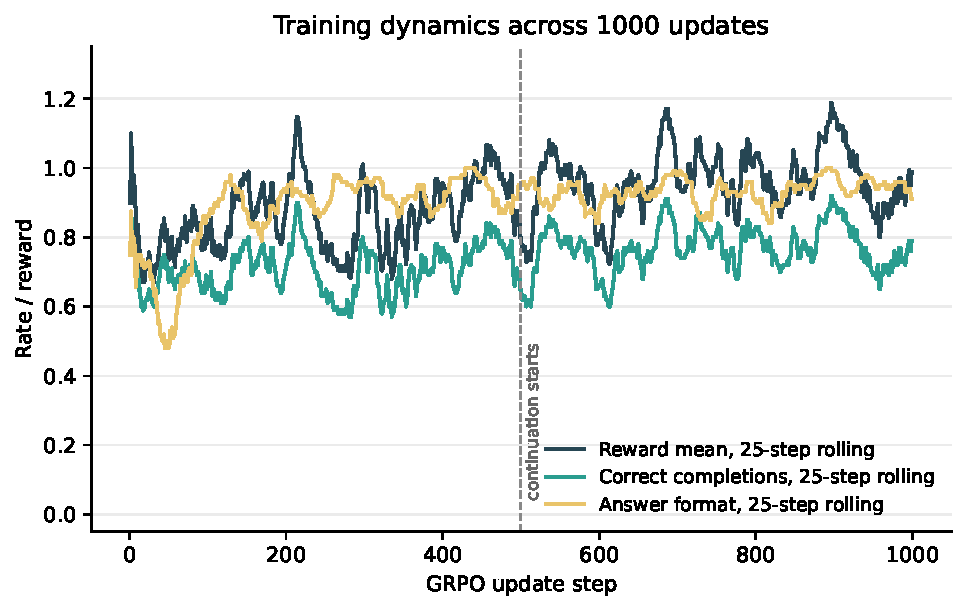
\includegraphics[width=0.95\linewidth]{figures/training_curves.pdf}
\caption{Rolling training curves across 1000 updates. The vertical line marks the transition from the first stage to continuation training.}
\end{figure}

\section{GRPO Signal Quality}

GRPO relies on relative reward within a group of completions. The most informative groups are those where some completions are correct and others are wrong. Saturated groups with 4/4 correct completions provide little math-correctness signal, though they can still reinforce formatting.

\begin{table}[h]
\centering
\caption{Group-level correctness distribution.}
\begin{tabular}{lrrrrrr}
\toprule
Run & 0/4 & 1/4 & 2/4 & 3/4 & 4/4 & Mixed groups \\
\midrule
GRPO-500 & 51 & 46 & 70 & 117 & 216 & 233/500 \\
Continuation & 33 & 34 & 59 & 101 & 273 & 194/500 \\
\bottomrule
\end{tabular}
\end{table}

The continuation run had more saturated 4/4-correct groups, which suggests the policy was already strong on many sampled prompts. This is consistent with the modest additional held-out gain from 70.0\% to 71.0\%.

\begin{figure}[h]
\centering
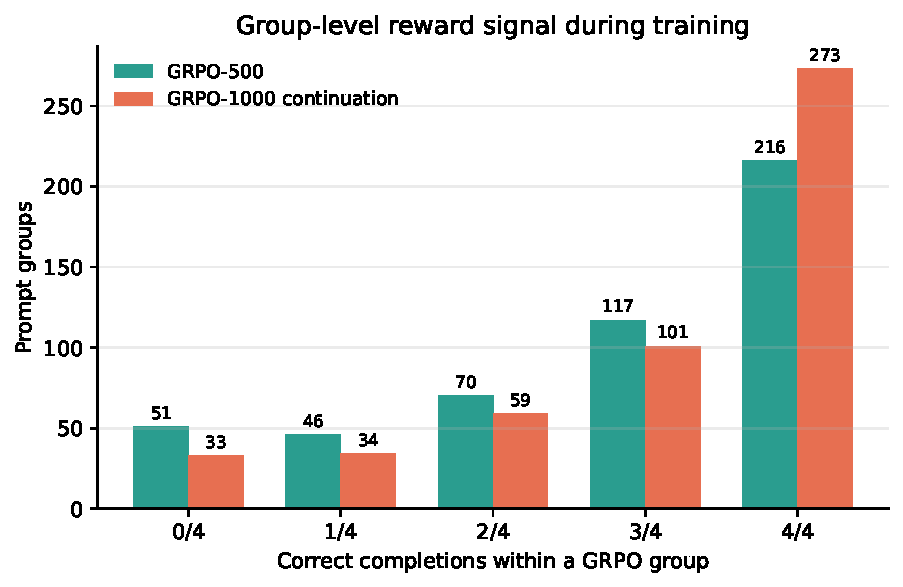
\includegraphics[width=0.84\linewidth]{figures/group_signal.pdf}
\caption{Correct completions per prompt group during training. Mixed groups are most useful for GRPO's relative advantage signal.}
\end{figure}

\section{Resource Profile}

The experiment fit comfortably on the Turing cluster's RTX 6000 Ada GPU. Peak logged memory was about 25.0 GiB in Stage 1 and 23.6 GiB in continuation, well below the 48 GiB device capacity. Peak logged temperature was 72 C.

\begin{figure}[h]
\centering
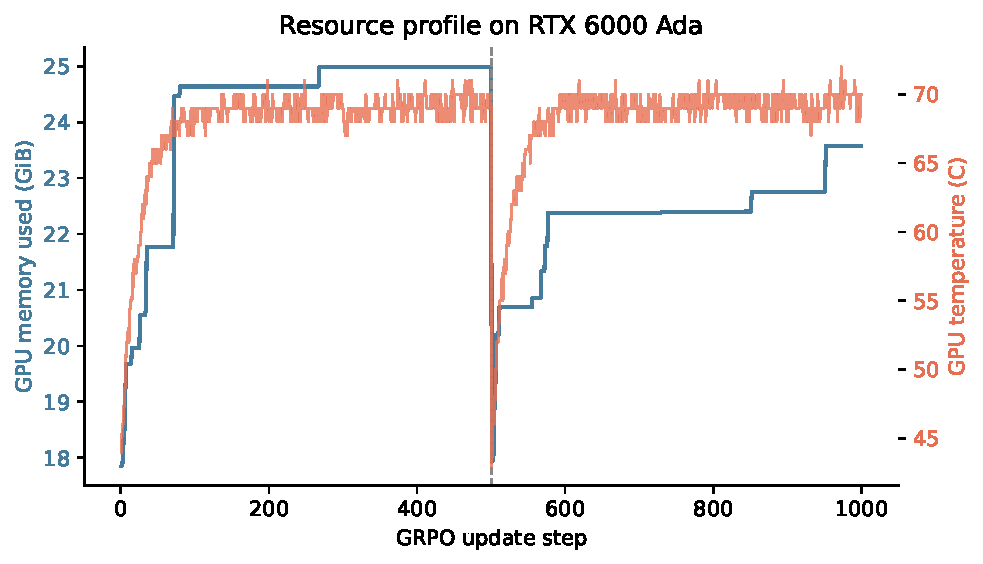
\includegraphics[width=0.90\linewidth]{figures/resource_profile.pdf}
\caption{GPU memory and temperature over the two training stages.}
\end{figure}

\section{Conclusion}

The 1000-update TinyGRPO-Math run produced a measurable pilot improvement over the base model:

\begin{itemize}
\item Accuracy improved from \textbf{66.5\%} to \textbf{71.0\%} on 200 held-out GSM8K test examples.
\item Final-answer format compliance improved from \textbf{77.5\%} to \textbf{97.5\%}.
\item Parseability stayed at \textbf{100\%}; truncation stayed at \textbf{0\%}.
\item The result was achieved with deterministic rule-based rewards, without training a reward model.
\end{itemize}

The strongest honest project claim is therefore: \emph{GRPO with deterministic math rewards improved held-out GSM8K accuracy by 4.5 percentage points and final-answer compliance by 20.0 percentage points for a compact 1.5B instruction model.} The main caveat is evaluation size: 200 examples is enough for a strong side-project demonstration, but not enough for a benchmark-quality statistical claim. A natural next step is to repeat the evaluation on the full GSM8K test split and run ablations over group size, KL strength, and reward composition.

\end{document}
